Un imagen $Q$ puede ser entendida como una función bidimensional $q(x,y)$ donde $x$ e $y$ son las coordenadas en el plano de cada elemento (los que serán llamados píxel) y la función da como resultado el nivel de gris o intensidad asociada a ese píxel. En concreto, cuando $x$ e $y$ así como la intensidad $q(x,y)$ son finitas y discretas hablaremos de que tenemos una imagen digital. Por eso mismo, el procesamiento digital de imagen se puede definir como aquel que se hace con imágenes digitales a través de un ordenador. Tiene su origen con la introducción de las primeras imágenes digitales a principios de 1920, donde se enviaban imágenes entre Londres y Nueva York por medio de un cable submarino.

Es claro que los seres humanos disponemos del sentido de la vista como el sentido más desarrollado para interacturar con el medio, pero esta está limitada a la banda visible dentro del espectro electromagnético. En cambio, el procesamiento digital de imagen puede cubrir el análisis de todo el espectro electromagnético, lo que incluye los ultrasonidos, el infrarojos, rayos X, etc. Esta es la principal razón por la que el procesamiento digital de imagen puede incluirse en una gran cantidad de campos.

Dentro del procesamiento de imagenes digitales se encuentra el campo de visión artificial. Esta es una subcampo de la inteligencia artificial (IA) y pretende conseguir emular la visión humana, incluyendo el poder aprender así como tomar en condideración entradas de un problema en forma de imagen. Actualmente, este campo está poco desarrollado \cite{lib:gonzalez} ya que el avance está siendo mucho más lento de lo que se esperaba en un primer momento. El área de análisis de imagen, que pretende entender cómo está formada la imagen, está situada a caballo entre la visión artificial y el procesamiento de imágen, y será esto lo que utilizaremos en este trabajo.

No hay una clara frontera entre el procesamiento y la visión artificial, esto hace que se hable de un paradigma que incluye 3 tipos de procesos; de bajo nivel, medio nivel y alto nivel. Dentro del nivel bajo se pueden incluir todos los procesos primitivos que tienen como objetivo reducir el ruido, ensalzar el contraste o ajustar la nitidez, por ejemplo. En un segundo nivel, más avanzado, se encuentran todos los procesos que tienen como entrada una imagen y obtienen atributos de esta. Pueden ser procesos como la segmentación (que se tratará aquí), descripción de objetos de la imagen o recocimiento de los mismos. En el último nivel se encuentran todas aquellas técnicas que hacen que todo ``tenga sentido'' ya que hacen que el análisis imite a la forma cognitiva de la mente humana.


\subsection{Imágenes digitales}
Como ya se ha explicado en el apartado anterior, se habla de imagen digital cuando se puede ser capaz de determinar todos sus elementos (píxeles), es decir, estos son de forma finita y discreta. A partir de esta idea, se dispone de dos formas de representación para las imágenes en niveles de gris, en los rangos $[0,1]\in\RR$ y $[0,255]\in\NN$. En el primer caso podremos decir que la imagen está normalizada. Además, todas las imágenes digitales serán representadas en una matriz que contendrá cada uno de sus píxeles de manera ordenada.


\begin{figure}
\centering
    \subfigure[Niveles de gris]
    {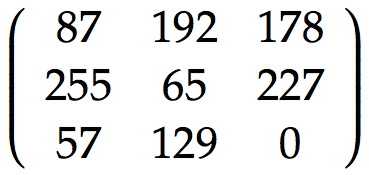
\includegraphics[height=0.1\textwidth]{img/matriznivelesgris.jpg}}\quad
    \subfigure[Normalizada]
    {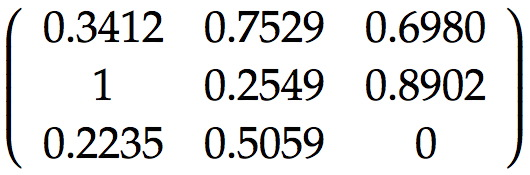
\includegraphics[height=0.1\textwidth]{img/matriznormalizada.jpg}}\quad\ 
    \subfigure[Gráfica]
    {
\includegraphics[width=0.1\textwidth]{img/imagendigital.jpg}}
    \caption{Imagen digital en diferentes representaciones.}
    \label{fig:defimagen}
\end{figure}

Como se puede apreciar en la figura \ref{fig:defimagen} cuanto más cercano a 0 sea el número, más negro será el nivel de gris, y cuanto más cercano a 1 ó 255, más blanco. En el caso de que quisieramos representar imágenes en color, utilizaríamos la forma RGB ({\em Red}, {\em Green} y {\em Blue}) donde existe una matriz como las anteriores por cada uno de los colores, donde al superponerlas se obtiene la imagen que vemos habitualmente.

\begin{definition}\label{def:histograma}
Se define el histograma de una imagen $Q$ con niveles de gris en el intervalo [0, 255] como la función $h(q) = n_q$ donde $n_q$ es el número de píxeles en la imagen con la intensidad $q$.
\end{definition}

Un ejemplo gráfico de la función de histograma para una imagen puede encontrarse en la figura \ref{img:rice}.


\subsection{Herramienta para el procesamiento digital: \MATLAB}
\MATLAB\ (abreviatura de {\em Matrix Laboratory}) es una herramienta de software matemático que ofrece un lenguaje de programación (lenguaje M) y un entorno de desarrollo integrado. Fue creado en 1984 por el informático y matemático Cleve Moler el cual buscaba una forma alternativa de ejecutar programas de álgebra en {\em Fortran}.

Entre sus pretaciones básica están la manipulación de matrices, la representación de datos y funciones o la implementación de algoritmos así como la creación de intrefaces de usuario (GUI). Además, el paquete básico de \MATLAB\ puede ser expandido por medio de {\em toolboxes}, como es el caso de este trabajo, donde se utilizará la relativa  a procesamiento de imagen. Se puede disponer también del software {\em Simulink} para trabajar conjuntamente a \MATLAB.

\subsection{Contraste}
Como en el trabajo se hace uso de imágenes con algo y bajo contraste, disponer una pequeña explicación. Pillar de los libros del laboratorio. \REV{Revisar}.

\subsection{Ruido en las imagenes}
Se condidera que una imagen está degradada cuando esta tiene ruido, esto es, cuando tiene defectos con respecto a la imagen que era realmente (fig. \ref{fig:defruido}). La principal fuente de ruido en images digitales se da en la adquisición o transmisión de las imagenes. Esto se puede deber a las condiciones ambientales o a la calidad de los sensores durante la toma de la imagen. Por ejemplo, la luminosidad, el polvo en el ambiente, etc. pueden ser determinantes. Por otra parte, en el caso de la transmisión estas pueden ser corrompidas por interferencias en el medio de transmisión, principalmente. Esto es claro cuando se transmite una imagen de un satelite, ya que la atmósfera interferir y provocar que la imagen recibida en la base terráquea no sea exactamente igual.
\begin{figure}
\centering
    \subfigure[Imagen original]
    {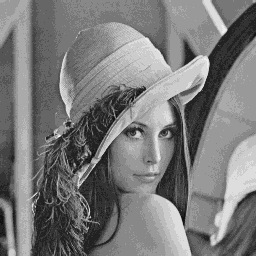
\includegraphics[width=0.3\textwidth]{img/lena}}\quad
    \subfigure[Imagen con ruido `sal y \mbox{pimienta}']
    {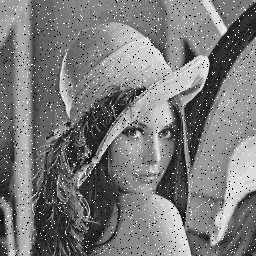
\includegraphics[width=0.3\textwidth]{img/lenas&p}}\quad
    \subfigure[Imagen con ruido gausiano]
    {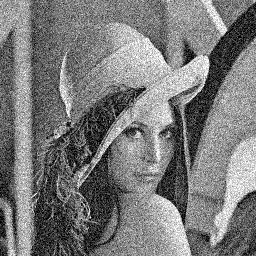
\includegraphics[width=0.3\textwidth]{img/lenaga}}
    \caption{Imagen de Lena con diferentes tipo de ruido}
    \label{fig:defruido}
\end{figure}

Las imágenes con ruido también se pueden crear artificialmente. Para ello utilizamos una cierta función $H$ de degradación, a la que añadimos un ruido al que llamaremos $\eta$ de forma que obtendremos una nueva imagen $g(x,y)$ que tendrá una serie de imperfecciones. Todo el ruido creado de esta forma se inflinjirá directamente sobre los píxeles de la imagen lo que probocará cambios en el histograma de la imagen en una forma u otra. Aun así, debemos tener en cuenta que no hay relación directa entre la intensidad nueva que tienen los píxeles y la anterior. 

Existen muchos tipos de ruido como el exponencial, el gamma, el uniforme, etc. pero en esta memoria se centra en los que se han utilizado, el gausiano y el de tipo `sal y pimienta'.

\subsubsection{Ruido gausiano}
Este puede ser uno de los modelos de ruido más utilizado en la práctica debido a que tiene una gran maleabilidad matemática. Basa su forma de actuar sobre la imagen en la función gausiana de probabilidad:
$$p(z) = \frac{1}{\sqrt{1}{2\pi\sigma}} e^\frac{-(z-\mu)^2}{2\sigma^2}$$
donde $z$ representa la intensidad, $\mu$ la media de $z$ y $\sigma$ la desviación estándar. Este tipo de ruido puede crearse en \MATLAB\ a través de la función \mintinline{matlab}{imnoise(img_var, 'gaussian')} sabiendo que \mintinline{matlab}{img_var} es la variable donde está almacenada la imagen en tipo \mintinline{matlab}{uint8}.

\subsubsection{Ruido de tipo `sal y pimienta'}
Este tipo de ruido, formalmente llamado impulsivo, hace que se conviertan píxeles de forma aleatoria en píxeles con intensidad 0 y 255. Esta es la razón de su particular nombre. De nuevo, fijándonos en \MATLAB, podremos crear imágenes con este tipo de ruido por medio del comando \mintinline{matlab}{imnoise(img_var, 'salt & pepper', prob_val)}, de nuevo \mintinline{matlab}{img_var} es la variable donde se almacena la imagen y \mintinline{matlab}{prob_val} es un valor entre 0 y 1 que hace las veces de probabilidad de la aparición del ruido. 

En este trabajo, se han utilizado imágenes con ruido para comprobar la adecuación o no de los algoritmos de segmentación al ruido. Ejemplos de ambos tipos de ruido se han presentado en la figura \ref{fig:defruido}.